\section{镜 (45pts)}
如图\ref{mirror} 所示,这道题是三个简单的几何光学问题。所有镜子的距离是\(d\),焦距是\(f\)或者\(-f\),设第一个物距为\(u\),请你回答下面的问题:
\begin{figure}[htbp]
	\centering
	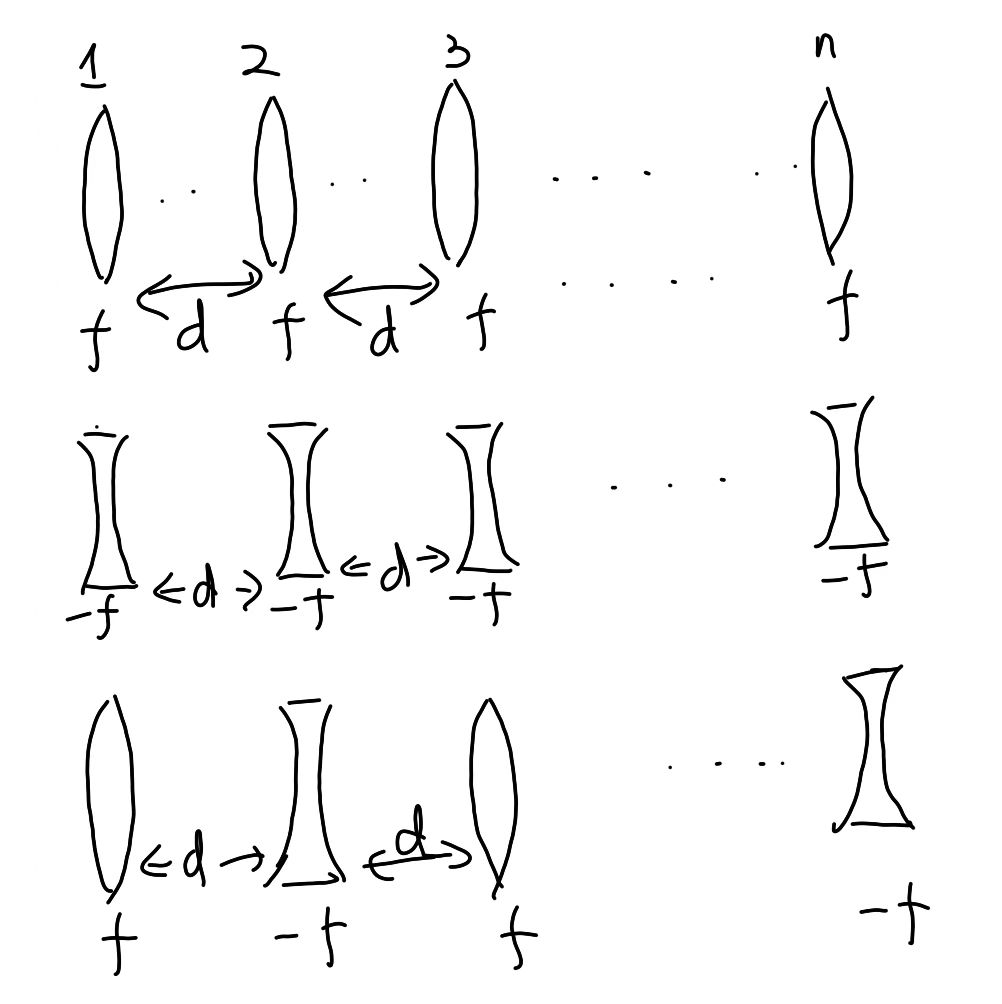
\includegraphics[width=0.5\textwidth]{mirror}
	\caption{这是三道摆放方案.}
	\label{mirror}
\end{figure}
\begin{enumerate}
	\item 光路全由凸透镜构成,总共\(n\)个凸透镜,求出最后的像距\(v\)与物距\(u\)的关系式。提示:你需要分两种情况讨论:\(d=4f\), \(d\neq 4f\)。 (30pts)
	\item 光路全由凹透镜构成,总共\(n\)个凹透镜,求出最后的像距\(v\)与物距\(u\)的关系式。(5pts)
	\item 光路全由凹透镜和凸透镜交替构成,总共\(n\)个透镜,得出相邻两项递推关系式给出计算方法即可(需要确保可以实现),无需给出具体答案(10pts) 
\end{enumerate}
